\documentclass{article}

% Use utf-8 encoding for foreign characters
\usepackage[utf8]{inputenc}

% Setup for fullpage use
\usepackage{fullpage}
\usepackage{graphicx}
\usepackage{hyperref}
\usepackage[french]{babel}
\usepackage[final]{pdfpages}
\usepackage{times}
\usepackage{gensymb}
\usepackage{color}
\usepackage{array}
\usepackage{textcomp}
\usepackage{subfig}
\usepackage{amsmath}
\usepackage{titlesec}
\usepackage{tabularx}
\includepdfset{pages = -, pagecommand = {}, scale = 0.9}
\setcounter{secnumdepth}{4}
\newcommand{\placeholder}[1]{{\noindent \color{red}[ #1 ]}}
\newtheorem{Rem}{Remarque}
\titleformat{\paragraph}
{\normalfont\normalsize\bfseries}{\theparagraph}{1em}{}
\titlespacing*{\paragraph}
{0pt}{3.25ex plus 1ex minus .2ex}{1.5ex plus .2ex}



\begin{document}


\title{
{\Huge Rapport du Projet\\
Statistique Multidimensionnelle\\
\smallskip
\author{
\textbf{Groupe Info n\degree 1}\\
JOSSE Thomas, HUYLENBROECK Florent, DELFOSSE Charly\\
}}
}
\date{Année Académique  2018-2019\\
 Bachelier en Sciences Informatiques
\\
\vspace{1cm}
Faculté des Sciences, UMons}



\maketitle            % typeset the title of the contribution
\bigskip
\begin{center} \today \end{center}
\begin{abstract}
Ce rapport est écrit dans le cadre du cours de \texttt{Statistique Multidimensionnelle} dispensé par M. \emph{Michel VOUÉ}. Ce projet consistait en l'application de l'\texttt{Analyse en Composantes Principales} vues au cours sur un cas concret, ainsi que la découverte d'une technique d'analyse non abordée au cours à savoir, l'\texttt{Analyse Discriminante Linéaire} ou ADL.
\end{abstract}
\newpage
\tableofcontents
\newpage
\section{Question 1 : ACP sur un cas concret}
\subsection{Introduction}
Pour cette question nous avions plusieurs sous-points à analyser: tout d'abord effectuer notre ACP des données à proprement dites, puis prédire à l'aide de notre analyse si le profil des données était stable et ensuite grouper les Provinces/Régions qui avaient des comportements similaires avec une méthode de classification hiérarchique ascendante. 

\subsection{ACP}
D'abord, les données ont été extraites et analysées. Les données représente l'évolution du pourcentage de chercheurs employés par les différentes provinces de Belgique.Un boxplot a été effectué avant et après centrage et réduction des données.

 \includegraphics[width=15cm,height=8cm]{"Boxplot1"}
 
On remarque que la moyenne et les quantiles ont tendance à augmenter au fil des années. Comme nous voulons utiliser l'analyse en composantes principales centrée réduite, nous devons centrer et réduire nos données, voici un boxplot des données après cette opération.

 \includegraphics[width=15cm,height=8cm]{"Boxplot2"} 
 
On peut déjà observer un aperçu du comportement des données d'une année à une autre. 

 \includegraphics[width=15cm,height=8cm]{"pairs"}
 
On remarque que les données ont l'air de suivre un modèle linéaire dans le temps, nous verrons par la suite si c'est réellement le cas. 

L'analyse en composante principale va permettre de mieux comprendre les données en réduisant le nombre de dimensions. Celle-ci va chercher un ou plusieurs axes ne passant plus forcèment par l'origine qui maximisent la distance entre tous les individus(dans notre cas les provinces)sur cet axe c'est à dire : $Max(H)(\sum_i^n \sum_j^n d_H^2(i,j))$ où n est le nombre d'individu, H l'axe en question et $d^2_H(i,j)$ la distance euclidienne entre 2 individus i et j sur l'axe H. Si $h_i$ est la projection de i sur l'axe H alors $d^2_H(i,j)=2n \sum_i^n (h_i - \bar{h})$ où $\bar{h}$ est la moyenne des projections de l'ensemble des individus sur H. On peut montrer que maximiser cette distance revient à maximiser la distance sur H entre tous les individus et le centre de gravité, on peut donc prendre celui-ci comme nouvelle origine et maximiser la distance des points à l'origine. Les nouvelles coordonnées des individus sont données par $x_{ij}=r_{ij} - \bar{r}_{ij}$. On décide ensuite de réduire nos données pour les mettre à l'échelle même si les variables ont les mêmes unités(pourcentages), on obtient donc les coordonnées centrées réduites : $x_{ij}=\frac{r_{ij} - \bar{r}_{ij}}{s_j \sqrt{n}}$ où $s_j$ est l'écart type de j.Après cette étape, nous voulons connaitre les similarités ou assimilarités entre la façon dont les variables varient les unes par rapport aux autres, pour se faire, la matrice de corrélation est calculée. la voici :
 
 \includegraphics[width=15cm,height=10cm]{"Corr"}
 
On remarque que toutes les correlations sont très proches de 1.Ceci s'explique par le fait que les données représentent l'évolution du pourcentage de chercheurs employés dans les différentes régions de Belgique au fil des ans. En effet, les valeurs de ce pourcentage d'une année à une autre sont fortement liées/correlées, la valeur de celui-ci à une année est basée sur sa valeur à l'année précédente et n'évolue pas drastiquement. La plus petite correlation est entre l'année 2008 et 2014, celle-ci vaut 0.915, ceci s'explique par le fait qu'il y a surement eu une inversion de tendance entre ces 2 années, que certaines villes ont eu un pourcentage plus élevé et l'inverse pour d'autres, par exemple le brabant wallon est passé de 1.55\% en 2008 à 3.1\% en 2014, la majorité des autres villes n'ont pas eu une telle augmentation.

Pour déterminer les composantes principales, c'est à dire les axes donnant la direction de la plus grande variance des données(vecteurs propres), il faut déterminer la portion de variance expliquée par chaque axe, ce n'est rien d'autres que les valeurs propres de la matrice de corrélation. Les voici :
\begin{table}[h]
\centering 
\begin{tabular}{|c|c|c|c|c|c|c|c|c|} 
  \hline
  8.806 & 0.128 & 0.04 & 0.02 & 0.004 & 0.001 & 0.0005 & 0.0001 & 0.00004 \\
  \hline
\end{tabular}
\end{table}
\newpage
On remarque la première valeur propre est bien plus grande que les autres, en réalité le premier axe représente 97.8\% du pourcentage de l'inertie, le 2e ne représente lui que 1.44\%. Le graphe ci-dessous illustre ce fait.

 \includegraphics[width=12cm,height=8cm]{"screebar"}
 
Pour connaitre le nombre de facteurs à retenir, il y a plusieurs critères possibles.  
Selon le critère de Kaiser, il faudrait retenir celle qui ont une valeur propre plus grande que 1, dans notre cas, il ne faudrait donc retenir que la première.
Un autre critère dit qu'il faut garder la valeur avant le "coude" c'est à dire l'éboulement dans le graphe de l'inertie que voici : 
 
  \includegraphics[width=12cm,height=8cm]{"screeplot"}
 
 
On remarque que le coude s'effectue entre la première et la deuxième valeur, selon ce critère il faudrait donc aussi ne garder que le premier facteur.
\\Pour appliquer l'analyse par composantes principales, il a donc été décidé de ne garder qu'une composante.
\\On obtient donc la seule composante principale, voici un tableau présentant les nouvelles coordonnées des variables sur cette composante(droite) par rapport leurs directions dans les anciens axes.
\begin{table}[h]
\centering 
\begin{tabular}{|c|c|c|} 
  \hline
  Variables & Nouvelles coord & Anciens axes\\
  \hline
  X2006 & -0.994 & -0.335\\
  \hline
  X2007 & -0.995 & -0.335\\
  \hline
  X2008 & -0.973 & -0.328\\
  \hline
  X2009 & -0.989 & -0.333\\
  \hline
  X2010 & -0.991 & -0.334\\
  \hline
  X2011 & -0.994 & -0.335\\
  \hline
  X2013 & -0.990 & -0.333\\
  \hline
  X2014 & -0.981 & -0.330\\
  \hline
  X2015 & -0.996 & -0.336\\
  \hline
\end{tabular}
\end{table}

Les coefficients de cette composante sont quasi identiques, ceci est le résultat du fait que toutes les variables sont fortement correlées à celle-ci. Toutes les variables sont très proches du cercle des corrélations comme elles valent presque toutes 1.

\\Sur les graphiques ci-dessous, pour chaque variable, on effectue une regression linéaire pour exprimer les valeurs initiales des individus en cette variable en fonction de leur valeurs dans la première composante. On remarque que pour toutes les variables, les points sont très proches de cette droite de regression, ceci explique le fait que la première composante explique tant de variance. La première composante suffit à elle toute seule pour résumer en une dimension toutes les informations.

	\includegraphics[width=10cm,height=7cm]{"score"} 
	
Les nouvelle coordonnées des individus sur cette composante peuvent être obtenues par la formule : $N_i=\sum_j^n u_j x_{ij}$ où n est le nombre de variables, $u_j$ est le $j^{eme}$ coefficient de la composante dans les anciens axes et $x_{ij}$ est $j^{eme}$ coordonnée de l'individu i dans les anciens axes(centré et réduit).On peut aussi déterminer la contribution de chaque individu à l'inertie de la composante par : $Cr(i)=N_i^2$.
\begin{table}[h]
\centering 
\begin{tabular}{|c|c|c|} 
  \hline
  Individus & Coordonées & Contribution(\%)\\
  \hline
  Bruxelles/Brussels Gewest & -3.472 & 12.443\\
  \hline  
  Antwerpen         &   -0.109    &    0.012\\
  \hline  
  Limburg (BE)       &     2.45   &   6.2\\
  \hline  
  Oost-Vlaanderen     &  -0.526   &    0.285\\
  \hline  
  Vlaams-Brabant       &  -3.896 &    15.673\\
  \hline  
  West-Vlaanderen     &   2.451  &     6.201\\
  \hline  
  Brabant Wallon     &   -5.773 &     34.407\\
  \hline
  Hainaut             &  2.296 &      5.44\\
  \hline  
  Liège              &  0.911  &     0.858\\
  \hline  
  Luxembourg (BE)     & 3.793 &      14.852\\
  \hline
  Namur              & 1.875   &      3.629\\
  \hline
\end{tabular}
\end{table}

 \newpage
\subsection{Le profil est-il stable dans le temps ?}

Le profil est stable car on a vu au point précédent que la matrice des correlations avaient des coefficients très proches de 1, donc en général aucune année n'a vraiment un comportement différent d'une autre dans les données, on a pas des changements imprévus c'est à dire une province qui verrait son pourcentage augmenter ou diminuer de façon inhabituelle d'une année à une autre. Le profil est donc stable dans le sens où dans le temps, celui-ci garde globalement le même comportement. 

\subsection{Groupement des Régions}
Avant de pouvoir classer les différentes régions/provinces en groupes, nous devons effectuer les calculs pour obtenir la matrice des distances.

La voici:\\
\begin{tabularx}{19cm}{|X|X|X|X|X|X|X|X|X|X|X|}
	\hline
	                   &Bruxelles / Brussels&Antwerpen &Limburg (BE) &Oost-Vlaanderen &Vlaams-Brabant &West-Vlaanderen &Brabant Wallon &Hainaut &Liège &Luxembourg (BE)\\
	\hline
	Antwerpen                           &2.1976387 &&&&&&&&&\\                                                                                                                             
	\hline
	Limburg (BE)                        &3.7924177       &1.6421791&&&&&&&&\\                                                                                                                                                         
	\hline
	Oost-Vlaanderen                     &1.8915634       &0.4301455          &1.9210062&&&&&&&\\                                                                                                                                      
	\hline
	Vlaams-Brabant                      &0.4977661       &2.4667642          &4.0669507             &2.1495597&&&&&&\\                                                                                                                
	\hline
	West-Vlaanderen                     &3.8006950       &1.6560244          &0.1286935             &1.9409271            &4.0820783 &&&&&\\                                                                                           
	\hline
	Brabant Wallon                      &1.9575174       &3.9798765          &5.5491930            & 3.6703024            &1.7755390             &5.5680656                                                                     &&&&\\
	\hline
	Hainaut                             &3.7125903       &1.5599647          &0.1778578            & 1.8341168            &3.9730810             &0.2564549            &5.4790390                                                &&&\\
	\hline
	Liège                               &2.8325198       &0.7078850          &0.9826074            & 0.9572507            &3.0928177             &1.0089326            &4.6193113     &0.8853731                                  &&\\
	\hline
	Luxembourg (BE)                     &4.7062104       &2.5412458          &0.9393496             &2.8423194            &4.9768604             &0.9233110            &6.4807544     &1.0232601   &1.8917065                      &\\
	\hline
	Namur                         &3.5118824       &1.4269053          &0.5102366             &1.6929400            &3.7991224             &0.5027041            &5.3359194     &0.4713670   &0.7868244             &1.2514964\\
	\hline
\end{tabularx}

Après avoir calculé ces distances, nous devions pouvoir trouver un moyen de regrouper ces distances pour pouvoir à la fin les classer en différents groupes. Pour cela, nous avons réalisé l'arbre des distances qui contient, sous forme d'arbre les relations entre chaque composante en fonction de sa distance par rapport aux autres. Le résultat est obtenu via l'algorithme suivant:

\begin{itemize}
	\item[Etape 1] n élément à classer
	\item[Etape 2] Calculer la matrice des distances et chercher les individus pour lesquels la distance est minimale. 
	Agréger ces éléments en un seul élément (ils seront frères dans l'arbre). On obtient à la fin une partition à n-1 éléments.
	\item[Etape 3] On recrée la matrice des distances avec ces modifications apportées et on boucle sur la 2$^{\text{ème}}$ étape jusqu'à ce que tous les individus soient contenus dans une seule classe (la racine de l'arbre).
\end{itemize}

A l'aide de cet algorithme nous avons obtenu cet arbre:

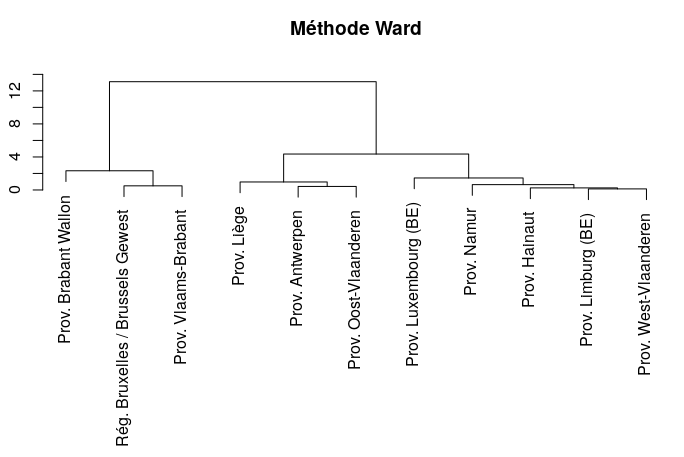
\includegraphics[width=12cm,height=7cm]{tree}

Pour réaliser celui-ci nous avons appliqué le critère de Ward généralisé qui dit que l'on doit rechercher les éléments pour lesquels la perte d'inertie interclasse est minimale.

\frame{$\Delta I_{ii'} = \frac{m_im_{i'}}{m_i + m_{i'}}d^2(x_i,x_{i'}$}

Maintenant que nous avons notre arbre des distances nous pouvons nous atteler à la tâche de diviser celui-ci en différentes classes. Comment faire cela ? Nous devons nous intéresser à la décroissance de l'inertie intraclasse. En effet, lorsque celle-ci diminue de manière plus faible cela veut dire que le nombre de groupe choisi est optimal.

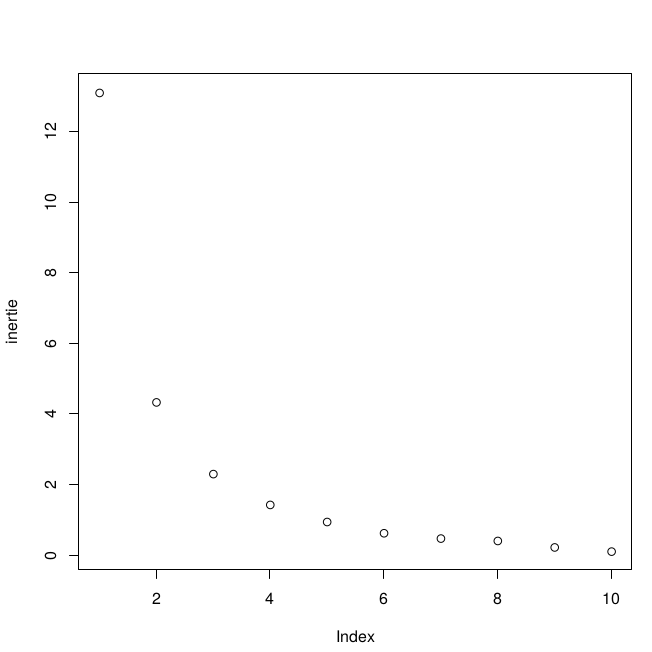
\includegraphics[width=10cm]{Inertie}
\newpage
D'après ce graphique, on pourrait classer nos individus en 5 groupes puisque c'est à ce niveau que l'inertie intraclasse se stabilise $\Rightarrow$ le critère d'optimalité.

Avec toutes ces données nous pouvons donner une forme finale à notre arbre des distances qui contiendra les différents groupes d'individus.

Le voici : 

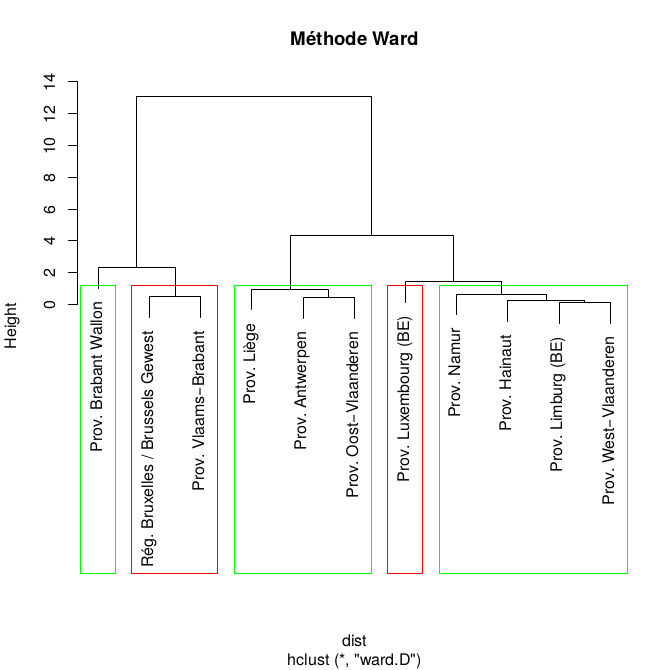
\includegraphics[width=\textwidth]{Ward}

Ce graphique nous montre la classification de nos régions qui ont les mêmes comportements au fur et à mesure du temps.

\section*{Q2 : L'analyse discriminante linéaire}
\subsection{Introduction}
L'analyse discriminante linéaire (\emph{ADL}) est une technique d'analyse discriminante prédictive. Son but es de pouvoir expliquer et prédire l'appartenance d'un individu à un groupe prédéfini à partir de caractéristiques qui ont été mesurées au préalable grâce à des varibles prédictives. Cette technique est comparable à la régression logistique.
\subsection{Fonctionnement}
Le principe de cette analyse est de calculer la distance entre $x$ (le vecteur des variables explicatives sur un individu que l'on veut classser) et chacun des $K$ centres de gravité des groupes $g_1,\ldots,g_K$ pour ensuite affecter $x$ au groupe le plus proche.\\
Cette distance peut être trouvée via la formule :
\[
	d^2(x,g_k) = (x - g_k)'\text{\bf W}^{-1}(x - g_k)\text{,}
\]
Où {\bf W} est la matrice des variance-covariance intra-groupe.\\
Pour cela, nous allons définir notre fonction linéaire discriminante du groupe $k$ pour savoir si $x$ appartient au groupe $k^*$ tel que :
\[
	k^* = arg \underset{k = 1,...,K}{max} d^2(x,g_k)
\]
que l'on peut réécrire:
\[
	k^* = arg \underset{k = 1,...,K}{max} L_K(x)
\]
où 
\[
	L_K(x) = x'\text{\bf W}^{-1}\text{\bf g}_k - \frac{1}{2}\text{\bf g}'_k\text{\bf W}^{-1}g_k
\]
Et $L_K(x)$ est notre fonction linéaire discriminante du groupe k.\\
Chaque $L_k(x)$ définit donc une fonction score qui donne une note représentant la probabilité d'appartenance au groupe de la fonction linéaire. $X$ est donc affecté au groupe dont le score est le plus élevé.
\subsection{Approche statistique}
\subsubsection{La règle bayesienne}
	Cette règle consiste à produire une estimation de la probabilité après notre affectation.
	Cela veut dire que nous devons réaliser une estimation pour une probabilité conditionnelle:
	\[
	P(Y = y_k | X) = \frac{P(Y = y_k) \times P(X| Y = y_k)}{\sum_{i=1}^{K} P(Y = y_i)\times P(X|Y = y_i)}
	\]
	
	Nous avons $P(Y = y_k)$ qui est la probabilité d'appartenance à la classe $y_k$ et $P(X|Y = y_k)$ qui est la fonction de densité des x par rapport à l'appartenance à la classe $y_k$.
	
	Et cette règle permet d'affecter une nouvelle observation x au groupe k* tel que:
	\[
		k^* = arg \underset{k=1,...,K}{max} P(Y = y_k | X)
	\] 
	\[
		k^*= arg \underset{k=1,...,K}{max} \pi_kf_k(x)
	\]	

\subsubsection{Hypothèse d'homoscédasticité}
L'homoscédasticité est le fait que les variances de chaque groupe soit équivalente (son contraire est l'hétéroscédasticité). Cela veut dire que les données sont réparties de la même manière autour de leur moyenne, ou centre de gravité. 
		
		Pour pouvoir effectuer de l'analyse discriminante linéaire c'est la principale hypothèse que l'on doit appliquer à nos données.
	
\subsubsection{Développement}
\noindent L'hypothèse respectée on peut réécrire la règle de Bayes telle que :
\[
	k^* = arg \underset{k=1,...,K}{max}x!\Sigma^{-1}\mu_k - \frac{1}{2}\mu'_k\Sigma^{-1}\mu_k + \ln(\pi_k)
\]
Il nous reste à estimer les  paramètres sur l'échantillon d'apprentissage:
\begin{itemize}
	\item $\mu_k$ est estimée par $g_k = \frac{1}{n_k}\sum_{i\in E_k}x_i$
	\item la matrice W avec $\Sigma$ commune à tous les groupes devient $\text{\bf W} = \frac{1}{n} \sum_{k=1}\sum_{i\in E_k}(x_i - \text{\bf g}_k)(x_i - \text{\bf g}_k)'$ avec biais ou sans biais :$$\text{\bf W} = \frac{1}{n - K}\sum_{k=1}\sum_{i\in E_k}x_i - \text{\bf g}_k)(x_i - \text{\bf g}_k)'$$
\end{itemize}
On obtient ainsi notre règle pour classifier nos individus par l'analyse discriminante linéaire:
\[
	k^* = arg \underset{k=1,...,K}{max}L_k(x)
\]
où
\[
			L_k(x) = x'\text{\bf W}^{-1}\text{\bf g}_k - \frac{1}{2}\text{\bf g}'_k\text{\bf W}^{-1}\text{\bf g}_k + \ln(\hat{\pi}_k)
		\] est la fonction linéaire discriminante du groupe $k$ et où $\hat{\pi}_k = \frac{n_k}{n}$. Elle fonctionne comme dans la règle géométrique.
		
\newpage
\section{Exemple}

Pour réaliser notre exemple, nous avons utiliser la fonction \texttt{discrimin} du package \texttt{ade4} de R qui nous a permis de réaliser l'analyse discriminante de la table de données "\emph{chazeb}" qui est fournie avec ce package ainsi que la table "\emph{skulls}" du même package.
\begin{figure}[h]
\centering
\includegraphics[scale=.33]{"LDA/Chazeb"}
\caption{Chazeb}

\includegraphics[scale=.33]{"LDA/Skulls"}
\caption{Skulls}
\end{figure}


\end{document}
